\documentclass[12pt,a4paper]{report}
\usepackage[margin=1in]{geometry}
 \geometry{a4paper, right=25mm, rmargin=0mm, outer=25mm, left=0mm, lmargin=0mm,  inner=25mm,
 top=0mm, tmargin=25mm, bottom=0mm, bmargin=25mm
}

%Packages
%\usepackage{sectsty}  % Gera warnings com o LuaTex
\usepackage[portuguese, english]{babel}
\usepackage{graphicx}
\usepackage{blindtext}
\usepackage{fontspec}
\usepackage{multirow}
\usepackage{afterpage}
\usepackage{layout}
\usepackage{blindtext}
\usepackage{fancyhdr}
\usepackage{xcolor}
\usepackage{color}
\usepackage{apacite}
\usepackage{caption}
\usepackage{fix-cm}
\usepackage{float}
\usepackage{makecell}
\usepackage{tabularx}
\usepackage{titlesec}
\usepackage{etoolbox}
\usepackage[acronym]{glossaries}
\usepackage{pdfpages}
\usepackage{longtable}

%Definições dos Títulos
\titleformat{\chapter}[display]
  {\normalfont\bfseries\color{darkgray}}{}{0pt}{\Large}
\titleformat*{\section}{\color{darkgray}\Large\bfseries}
\titleformat*{\subsection}{\color{darkgray}\Large\bfseries\color{darkgray}}
\titleformat*{\subsubsection}{\color{darkgray}\Large\bfseries}
\setcounter{secnumdepth}{3}
\renewcommand{\thesubsubsection}{\alph{subsubsection})}

%Definições do Documento
\renewcommand{\baselinestretch}{1.5} 
\setmainfont{NewsGotT.ttf}
\setmainfont[
%Mapping=tex-text,  %Gera warning com LuaTex
Ligatures=TeX,
AutoFakeSlant=0.20,
BoldFont=NewsGotTBold.ttf
]{NewsGotT.ttf} 

\titlespacing{\chapter}{0pt}{-40pt}{10pt} 


%Definições do Cabeçalho
\fancyhf{}
\renewcommand{\chaptermark}[1]{\markboth{#1}{}}
\renewcommand{\sectionmark}[1]{\markright{#1}{}}
\fancyhead[R]{\textcolor{gray}{Análise Crítica de Modelos Simples para a Abordagem à Cibersegurança e Privacidade }} 

%Definições das Secções
\fancyhead[L]{}
\setlength{\headheight}{15pt}
\pagestyle{fancy}
\patchcmd{\chapter}{\thispagestyle{plain}}{\thispagestyle{fancy}}{}{}
\patchcmd{\headrule}{\hrule}{\color{black}\hrule}{}{} %Change color Hrule


\begin{document}
\fancyfoot[R]{\thepage}
\pagenumbering{roman}

%Capa 
\begin{titlepage}
    
\includepdf[pages={1}]{chapter/pdf/capaTP3.pdf}
\end{titlepage}


%Índice
\renewcommand{\contentsname}{Índice}
\tableofcontents
\clearpage
\let\oldnumberline\numberline% Copy \numberline into \oldnumberline
\renewcommand{\numberline}[1]{\hspace*{-1.5em}}% Remove number argument


%Definições do Rodapé
\fancyfoot[R]{\thepage}

%Enquadramento
\setcounter{chapter}{1}
\chapter*{\thechapter \quad Enquadramento e Motivação}
\addcontentsline{toc}{chapter}{\thechapter \quad Enquadramento e Motivação}
\pagenumbering{arabic}
\paragraph{}
Lorem ipsum dolor sit amet, consectetur adipiscing elit. Donec eget dictum erat. Vestibulum ante ipsum primis in faucibus orci luctus et ultrices posuere cubilia curae; Nunc placerat turpis magna, eu tempus risus finibus vitae. Donec at nunc posuere, porta sem et, congue erat. Aenean suscipit faucibus scelerisque. Aenean in odio elementum, blandit tellus et, convallis nisl. Suspendisse ut nisi at augue tristique tempus. Cras lobortis arcu in felis pulvinar convallis. Aliquam sollicitudin neque non elementum iaculis. Pellentesque mattis sapien a justo pellentesque, ut ornare mauris accumsan. Nulla facilisi. Maecenas posuere luctus ipsum, a faucibus enim lacinia et. Nulla id vehicula urna, vitae feugiat arcu. Nulla laoreet libero quam, quis varius odio egestas vel. Fusce tempus orci nec ligula aliquam, aliquet aliquam ex dictum. Nullam pharetra tincidunt tellus, quis facilisis nisl luctus sit amet.

Phasellus gravida mi nec tristique pharetra. Mauris feugiat condimentum convallis. Sed hendrerit erat at dui congue, a ultrices nulla tincidunt. Aenean sed dolor interdum, laoreet lectus in, placerat libero. Mauris elementum gravida sem, sit amet posuere erat fringilla eu. Mauris sit amet ex interdum orci aliquam efficitur et id mi. Nulla posuere nec odio sed cursus. Donec dictum ex vel magna maximus faucibus. Suspendisse in tincidunt odio. Donec tellus risus, rhoncus quis fermentum id, tincidunt id lorem. Quisque tincidunt luctus massa, vel convallis arcu tincidunt vitae. Proin dignissim purus eget cursus aliquam.

There are many variations of passages of Lorem Ipsum available, but the majority have suffered alteration in some form, by injected humour, or randomised words which don't look even slightly believable. If you are going to use a passage of Lorem Ipsum, you need to be sure there isn't anything embarrassing hidden in the middle of text. All the Lorem Ipsum generators on the Internet tend to repeat predefined chunks as necessary, making this the first true generator on the Internet. It uses a dictionary of over 200 Latin words, combined with a handful of model sentence structures, to generate Lorem Ipsum which looks reasonable. The generated Lorem Ipsum is therefore always free from repetition, injected humour, or non-characteristic words etc. %Added from chapter directory

%\newpage\null\thispagestyle{empty}\newpage

%Objetivos e Resultados Esperados
\setcounter{chapter}{2}
\setcounter{section}{0}
\chapter*{\thechapter \quad Objetivos e Resultados Esperados}
\addcontentsline{toc}{chapter}{\thechapter \quad Objetivos e Resultados Esperados}
\paragraph{}

Dentro deste projeto de LaTeX e Git , os 4 membros do grupo irão ter como objetivos o seguinte:
\begin{itemize}
   \item Desenvolvimento de uma template de relatório em LaTeX;
   \item Utilização da ferramenta \textit{GIT} para o desenvolvimento deste relatório em conjunto;
   \item Promoção de trabalho em grupo;
\end{itemize}




%Estado da Arte
\setcounter{chapter}{3}
\setcounter{section}{0}
\chapter*{\thechapter \quad Estado da Arte}
\addcontentsline{toc}{chapter}{\thechapter \quad Estado da Arte}
\paragraph{}
Segundo \cite{Mascetti2018}



%Caso de Estudo
\setcounter{chapter}{4}
\setcounter{section}{0}
\chapter*{\thechapter \quad Caso de Estudo}
\addcontentsline{toc}{chapter}{\thechapter \quad Caso de Estudo}
\paragraph{}
Algum texto



%Bibliografia
\renewcommand\bibname{Referências Bibliográficas}
\bibliographystyle{apacite}
\bibliography{mybib.bib}

%Anexos
\addcontentsline{toc}{chapter}{Calendarização}

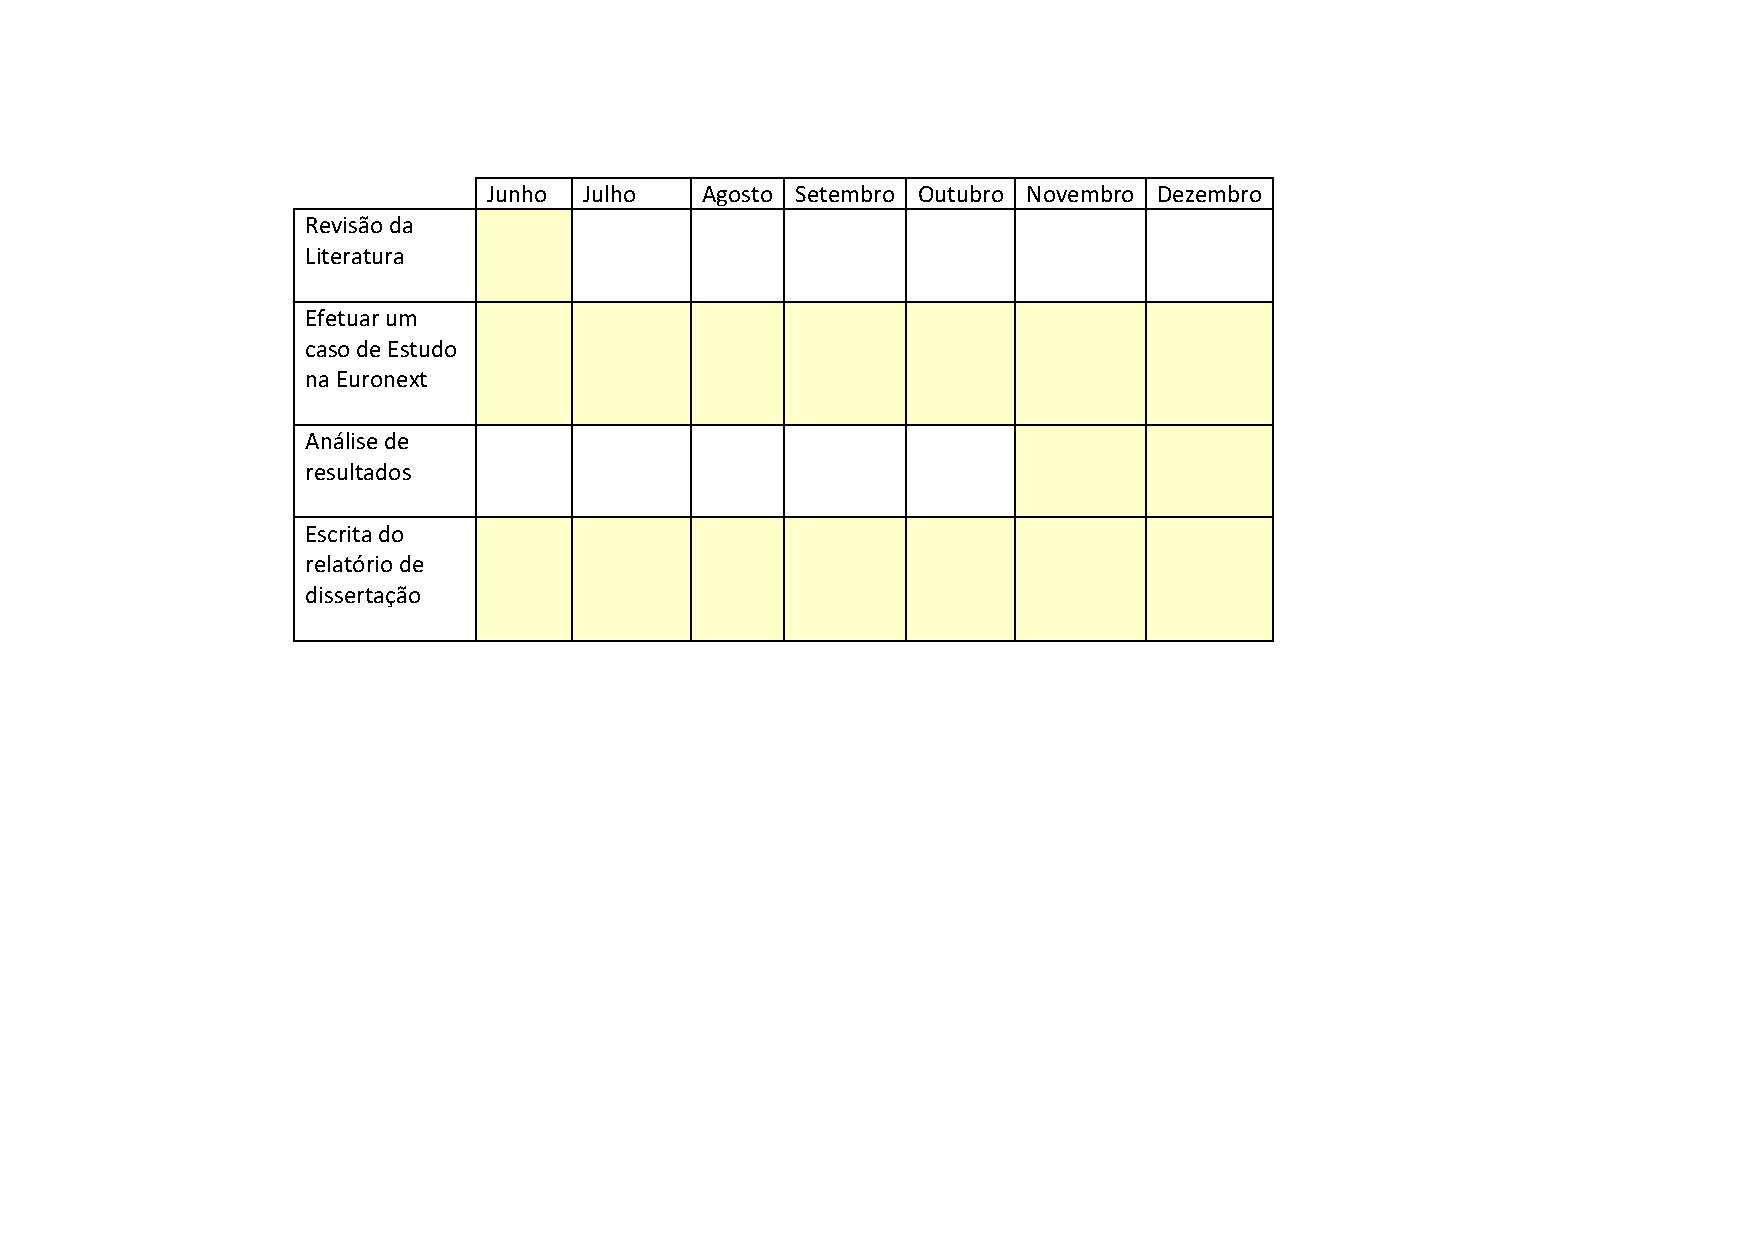
\includepdf[pages=-,angle=0]{chapter/pdf/Plano_de_Atividades.pdf}

\end{document}  